\PassOptionsToPackage{unicode=true}{hyperref} % options for packages loaded elsewhere
\PassOptionsToPackage{hyphens}{url}
\PassOptionsToPackage{dvipsnames,svgnames*,x11names*}{xcolor}
%
\documentclass[ignorenonframetext,]{beamer}
\usepackage{pgfpages}
\setbeamertemplate{caption}[numbered]
\setbeamertemplate{caption label separator}{: }
\setbeamercolor{caption name}{fg=normal text.fg}
\beamertemplatenavigationsymbolsempty
% Prevent slide breaks in the middle of a paragraph:
\widowpenalties 1 10000
\raggedbottom
\setbeamertemplate{part page}{
\centering
\begin{beamercolorbox}[sep=16pt,center]{part title}
  \usebeamerfont{part title}\insertpart\par
\end{beamercolorbox}
}
\setbeamertemplate{section page}{
\centering
\begin{beamercolorbox}[sep=12pt,center]{part title}
  \usebeamerfont{section title}\insertsection\par
\end{beamercolorbox}
}
\setbeamertemplate{subsection page}{
\centering
\begin{beamercolorbox}[sep=8pt,center]{part title}
  \usebeamerfont{subsection title}\insertsubsection\par
\end{beamercolorbox}
}
\AtBeginPart{
  \frame{\partpage}
}
\AtBeginSection{
  \ifbibliography
  \else
    \frame{\sectionpage}
  \fi
}
\AtBeginSubsection{
  \frame{\subsectionpage}
}
\usepackage{lmodern}
\usepackage{amssymb,amsmath}
\usepackage{ifxetex,ifluatex}
\usepackage{fixltx2e} % provides \textsubscript
\ifnum 0\ifxetex 1\fi\ifluatex 1\fi=0 % if pdftex
  \usepackage[T1]{fontenc}
  \usepackage[utf8]{inputenc}
  \usepackage{textcomp} % provides euro and other symbols
\else % if luatex or xelatex
  \usepackage{unicode-math}
  \defaultfontfeatures{Ligatures=TeX,Scale=MatchLowercase}
\fi
% use upquote if available, for straight quotes in verbatim environments
\IfFileExists{upquote.sty}{\usepackage{upquote}}{}
% use microtype if available
\IfFileExists{microtype.sty}{%
\usepackage[]{microtype}
\UseMicrotypeSet[protrusion]{basicmath} % disable protrusion for tt fonts
}{}
\IfFileExists{parskip.sty}{%
\usepackage{parskip}
}{% else
\setlength{\parindent}{0pt}
\setlength{\parskip}{6pt plus 2pt minus 1pt}
}
\usepackage{xcolor}
\usepackage{hyperref}
\hypersetup{
            pdftitle={Introduction to R Programming},
            pdfauthor={Pedro Fonseca},
            colorlinks=true,
            linkcolor=Maroon,
            filecolor=Maroon,
            citecolor=Blue,
            urlcolor=blue,
            breaklinks=true}
\urlstyle{same}  % don't use monospace font for urls
\newif\ifbibliography
\usepackage{color}
\usepackage{fancyvrb}
\newcommand{\VerbBar}{|}
\newcommand{\VERB}{\Verb[commandchars=\\\{\}]}
\DefineVerbatimEnvironment{Highlighting}{Verbatim}{commandchars=\\\{\}}
% Add ',fontsize=\small' for more characters per line
\usepackage{framed}
\definecolor{shadecolor}{RGB}{248,248,248}
\newenvironment{Shaded}{\begin{snugshade}}{\end{snugshade}}
\newcommand{\AlertTok}[1]{\textcolor[rgb]{0.94,0.16,0.16}{#1}}
\newcommand{\AnnotationTok}[1]{\textcolor[rgb]{0.56,0.35,0.01}{\textbf{\textit{#1}}}}
\newcommand{\AttributeTok}[1]{\textcolor[rgb]{0.77,0.63,0.00}{#1}}
\newcommand{\BaseNTok}[1]{\textcolor[rgb]{0.00,0.00,0.81}{#1}}
\newcommand{\BuiltInTok}[1]{#1}
\newcommand{\CharTok}[1]{\textcolor[rgb]{0.31,0.60,0.02}{#1}}
\newcommand{\CommentTok}[1]{\textcolor[rgb]{0.56,0.35,0.01}{\textit{#1}}}
\newcommand{\CommentVarTok}[1]{\textcolor[rgb]{0.56,0.35,0.01}{\textbf{\textit{#1}}}}
\newcommand{\ConstantTok}[1]{\textcolor[rgb]{0.00,0.00,0.00}{#1}}
\newcommand{\ControlFlowTok}[1]{\textcolor[rgb]{0.13,0.29,0.53}{\textbf{#1}}}
\newcommand{\DataTypeTok}[1]{\textcolor[rgb]{0.13,0.29,0.53}{#1}}
\newcommand{\DecValTok}[1]{\textcolor[rgb]{0.00,0.00,0.81}{#1}}
\newcommand{\DocumentationTok}[1]{\textcolor[rgb]{0.56,0.35,0.01}{\textbf{\textit{#1}}}}
\newcommand{\ErrorTok}[1]{\textcolor[rgb]{0.64,0.00,0.00}{\textbf{#1}}}
\newcommand{\ExtensionTok}[1]{#1}
\newcommand{\FloatTok}[1]{\textcolor[rgb]{0.00,0.00,0.81}{#1}}
\newcommand{\FunctionTok}[1]{\textcolor[rgb]{0.00,0.00,0.00}{#1}}
\newcommand{\ImportTok}[1]{#1}
\newcommand{\InformationTok}[1]{\textcolor[rgb]{0.56,0.35,0.01}{\textbf{\textit{#1}}}}
\newcommand{\KeywordTok}[1]{\textcolor[rgb]{0.13,0.29,0.53}{\textbf{#1}}}
\newcommand{\NormalTok}[1]{#1}
\newcommand{\OperatorTok}[1]{\textcolor[rgb]{0.81,0.36,0.00}{\textbf{#1}}}
\newcommand{\OtherTok}[1]{\textcolor[rgb]{0.56,0.35,0.01}{#1}}
\newcommand{\PreprocessorTok}[1]{\textcolor[rgb]{0.56,0.35,0.01}{\textit{#1}}}
\newcommand{\RegionMarkerTok}[1]{#1}
\newcommand{\SpecialCharTok}[1]{\textcolor[rgb]{0.00,0.00,0.00}{#1}}
\newcommand{\SpecialStringTok}[1]{\textcolor[rgb]{0.31,0.60,0.02}{#1}}
\newcommand{\StringTok}[1]{\textcolor[rgb]{0.31,0.60,0.02}{#1}}
\newcommand{\VariableTok}[1]{\textcolor[rgb]{0.00,0.00,0.00}{#1}}
\newcommand{\VerbatimStringTok}[1]{\textcolor[rgb]{0.31,0.60,0.02}{#1}}
\newcommand{\WarningTok}[1]{\textcolor[rgb]{0.56,0.35,0.01}{\textbf{\textit{#1}}}}
\setlength{\emergencystretch}{3em}  % prevent overfull lines
\providecommand{\tightlist}{%
  \setlength{\itemsep}{0pt}\setlength{\parskip}{0pt}}
\setcounter{secnumdepth}{0}

% set default figure placement to htbp
\makeatletter
\def\fps@figure{htbp}
\makeatother


\title{Introduction to R Programming}
\providecommand{\subtitle}[1]{}
\subtitle{Getting Started}
\author{Pedro Fonseca}
\date{01 Maio 2020}

\begin{document}
\frame{\titlepage}

\begin{frame}{R and Rstudio}
\protect\hypertarget{r-and-rstudio}{}

\begin{itemize}
\tightlist
\item
  R is a programming language and free software environment for
  statistical computing and graphics.
\item
  RStudio is an integrated development environment (IDE) for R.
\item
  You can use R without using RStudio, but you can't use Rstudio without
  using R.
\end{itemize}

\end{frame}

\begin{frame}{This is how R looks like}
\protect\hypertarget{this-is-how-r-looks-like}{}

\begin{figure}
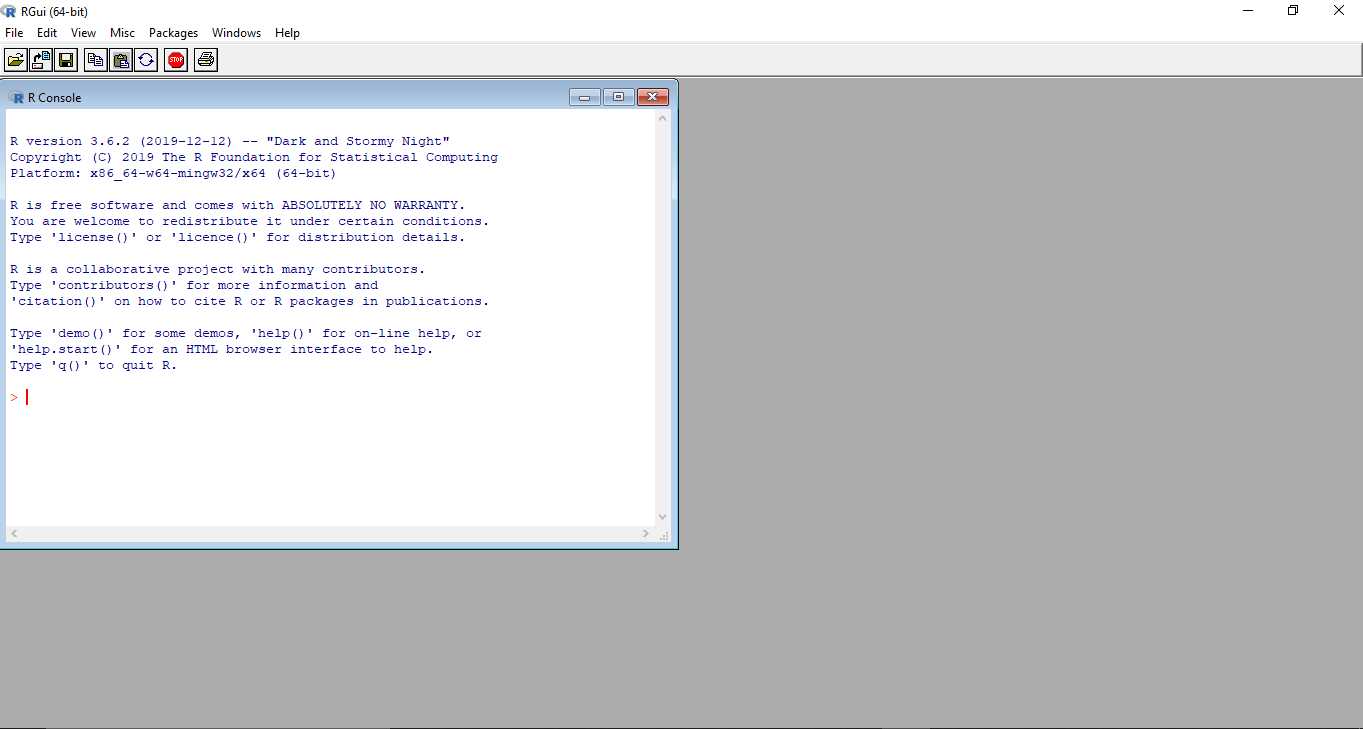
\includegraphics[scale = .3]{figures/Screenshot_1}
\caption{R console on windows}
\end{figure}

\end{frame}

\begin{frame}{This is how R looks like}
\protect\hypertarget{this-is-how-r-looks-like-1}{}

\begin{figure}
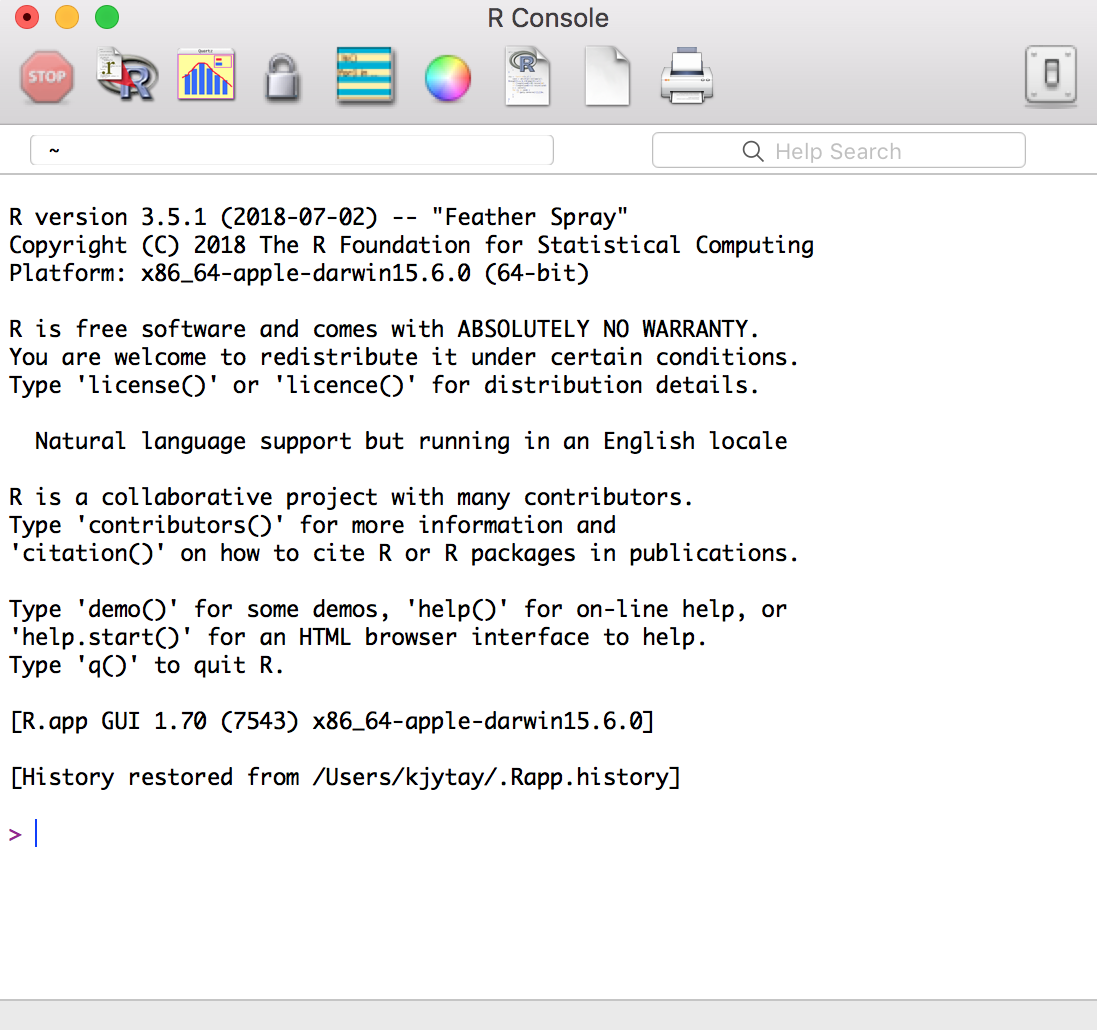
\includegraphics[scale = .35]{figures/r-mac.png}
\caption{R console on MacOS}
\end{figure}

\end{frame}

\begin{frame}{This is how R looks like}
\protect\hypertarget{this-is-how-r-looks-like-2}{}

\begin{figure}
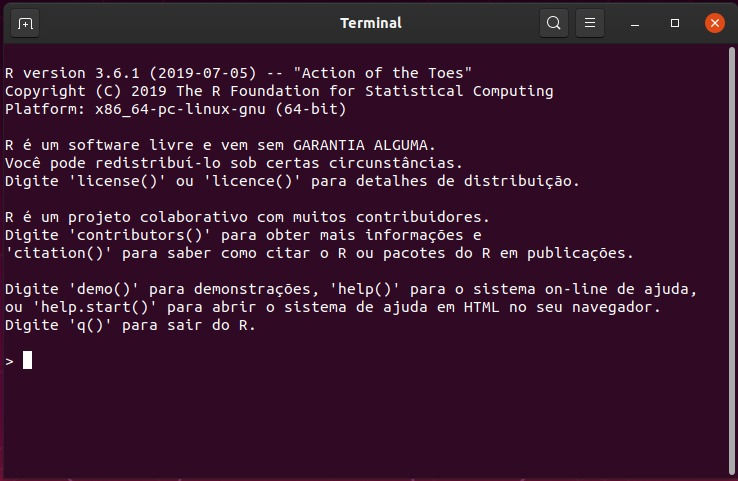
\includegraphics[scale = .3]{figures/r-linux}
\caption{R on Ununtu}
\end{figure}

\end{frame}

\begin{frame}{This is how Rstudio looks like}
\protect\hypertarget{this-is-how-rstudio-looks-like}{}

\begin{figure}[H]
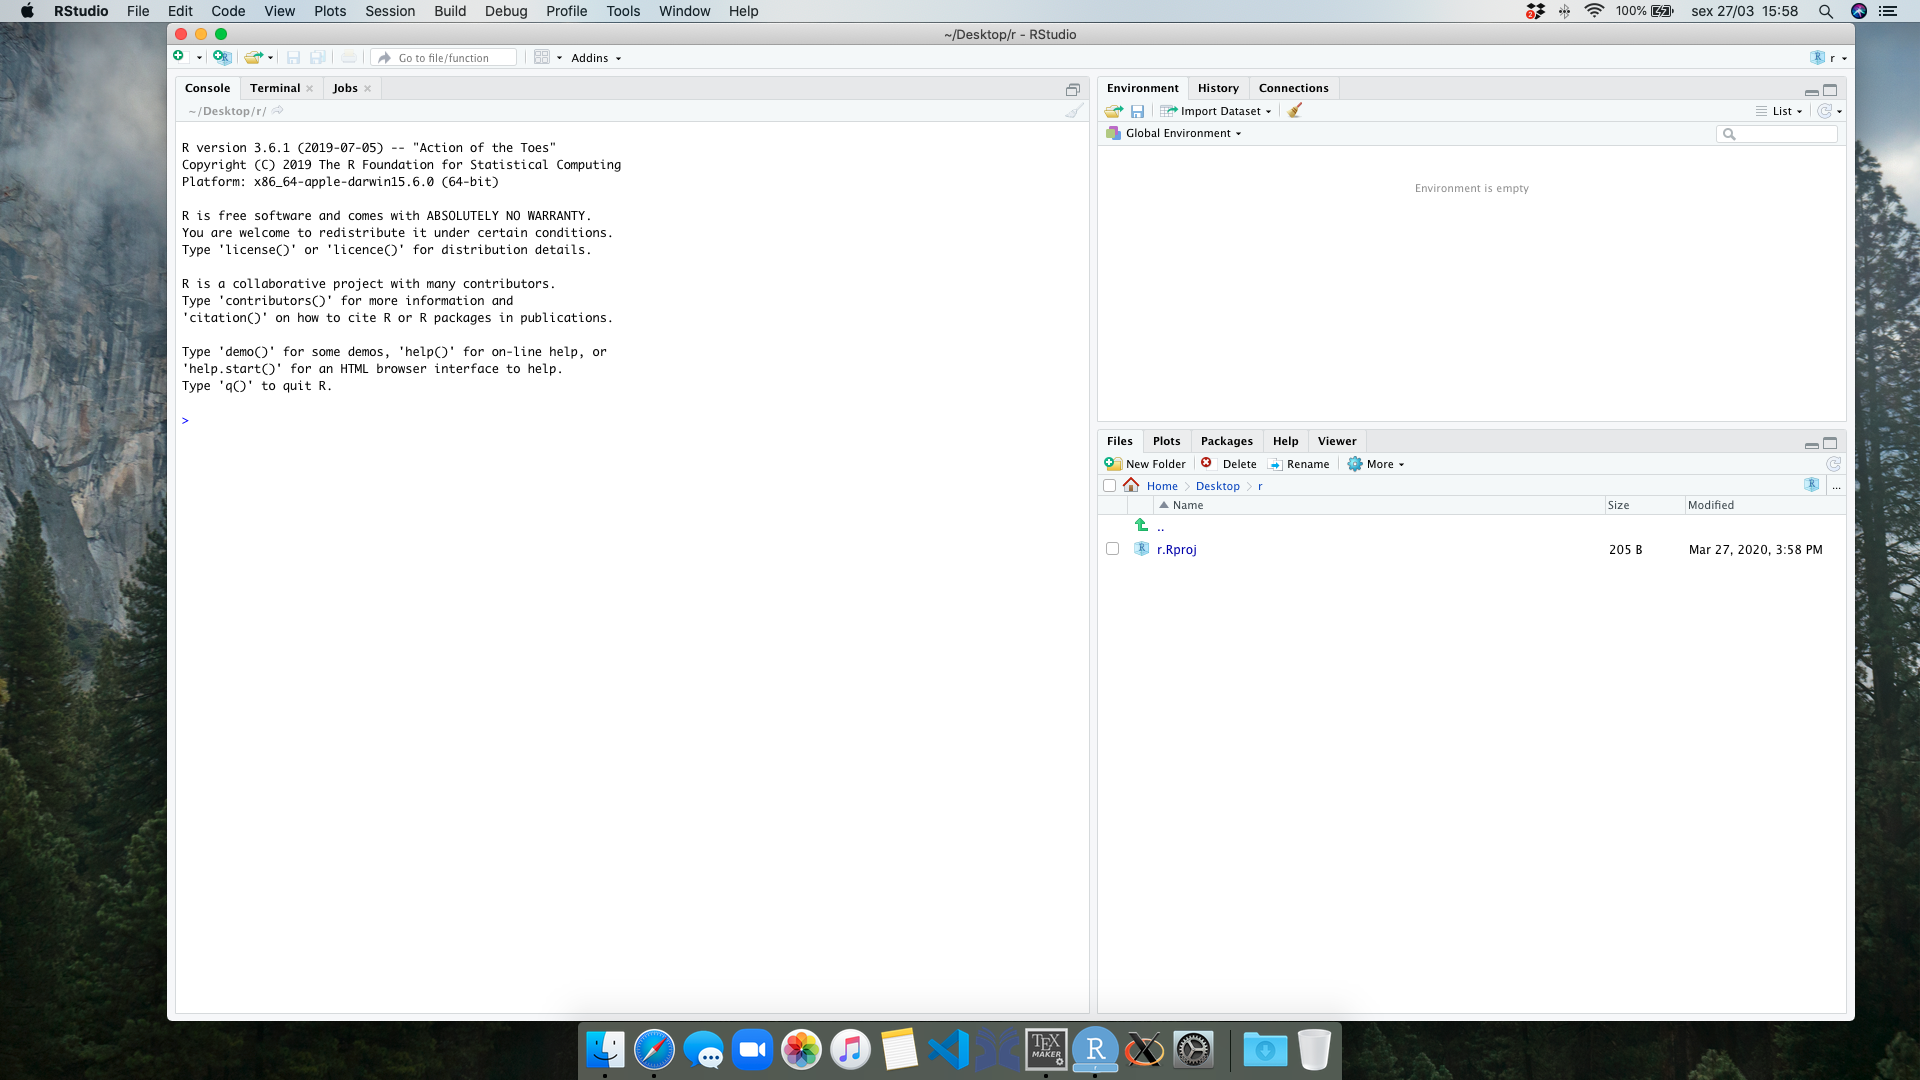
\includegraphics[scale = 0.15]{figures/Screenshot_mac}%
\caption{Rstudio on MacOS}
\end{figure}

\end{frame}

\begin{frame}{Rstudio Cloud}
\protect\hypertarget{rstudio-cloud}{}

If you don't want to install R and RStudio:

\begin{enumerate}
\item
  Go to \href{https://rstudio.cloud/}{RStudio Cloud}
\item
  Create an account and login
\item
  Click ``New Project''
\end{enumerate}

\end{frame}

\begin{frame}{Rstudio Cloud}
\protect\hypertarget{rstudio-cloud-1}{}

\begin{figure}[H]
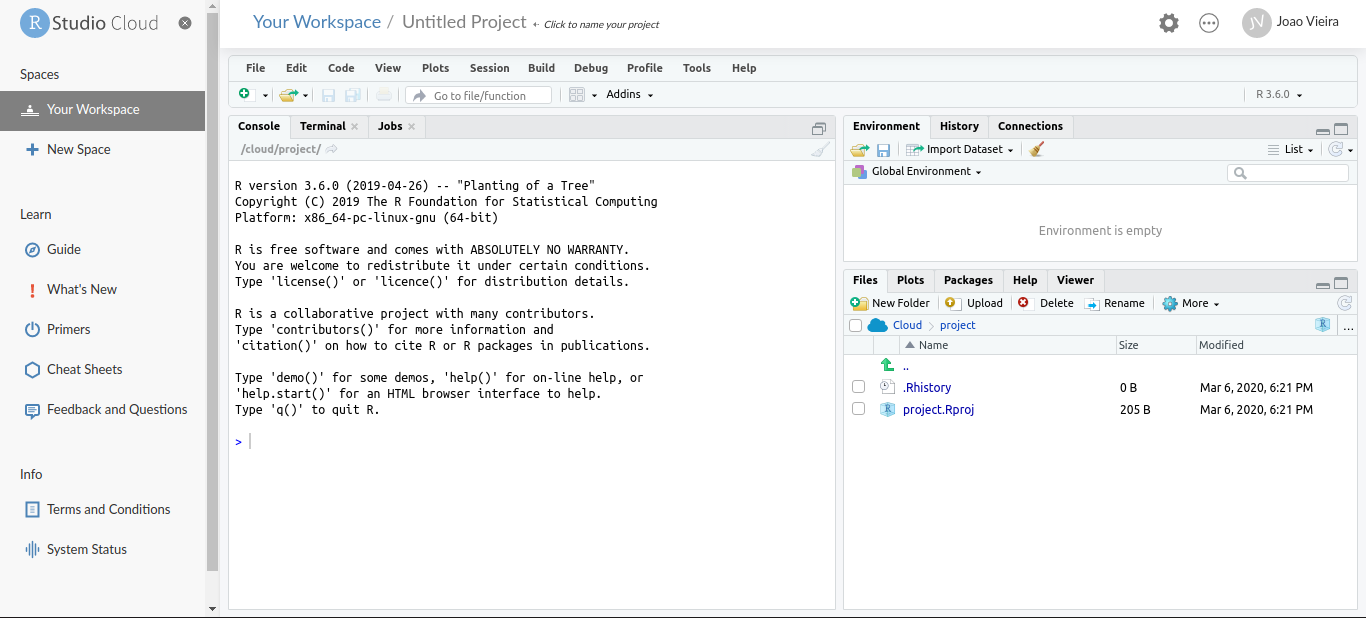
\includegraphics[scale = .3]{figures/Screenshot_6} 
\caption{Rstudio Cloud}
\end{figure}

For additional information see \url{https://rstudio.cloud/learn/guide}

\end{frame}

\begin{frame}{Your first Rstudio project}
\protect\hypertarget{your-first-rstudio-project}{}

\begin{figure}
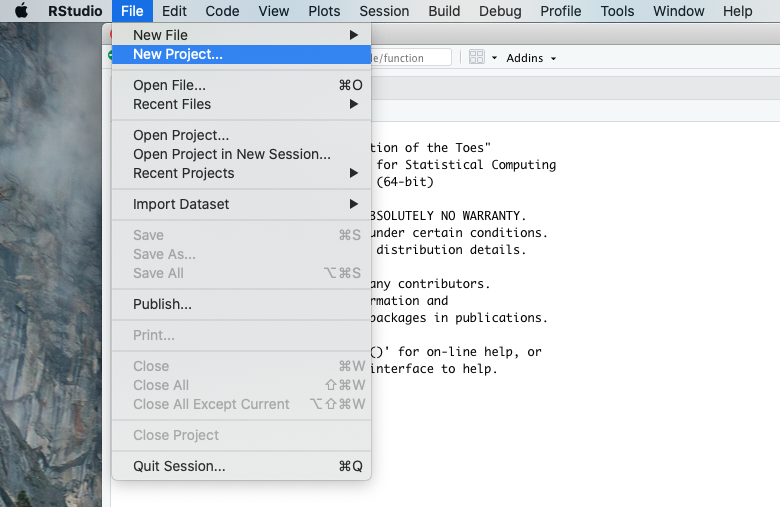
\includegraphics[scale=0.35]{figures/new-project-1.png}
\end{figure}

\end{frame}

\begin{frame}{Your first Rstudio project}
\protect\hypertarget{your-first-rstudio-project-1}{}

\begin{figure}
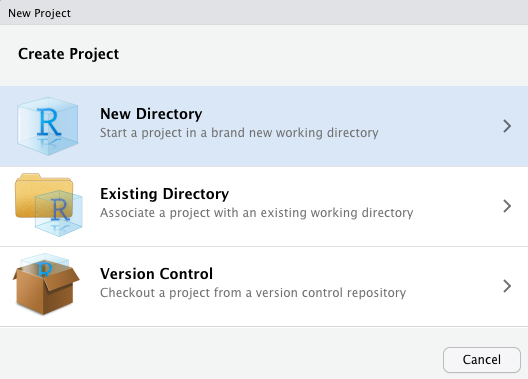
\includegraphics[scale=0.43]{figures/new-project-2.png}
\end{figure}

\end{frame}

\begin{frame}{Your first Rstudio project}
\protect\hypertarget{your-first-rstudio-project-2}{}

\begin{figure}
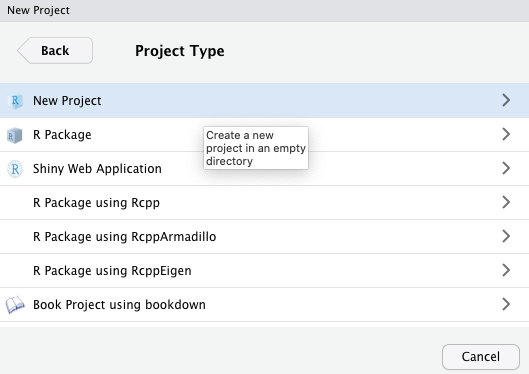
\includegraphics[scale=0.43]{figures/new-project-3.png}
\end{figure}

\end{frame}

\begin{frame}{Your first Rstudio project}
\protect\hypertarget{your-first-rstudio-project-3}{}

\begin{figure}
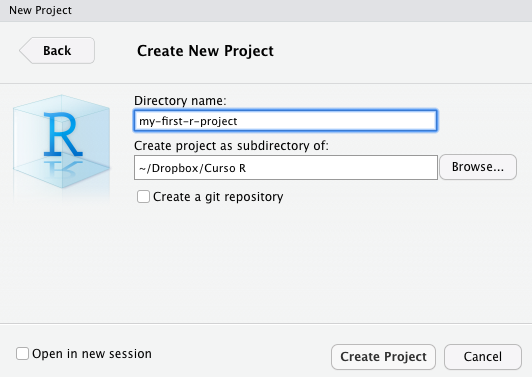
\includegraphics[scale=0.43]{figures/new-project-4.png}
\end{figure}

\end{frame}

\begin{frame}{Your first Rstudio project}
\protect\hypertarget{your-first-rstudio-project-4}{}

\begin{figure}
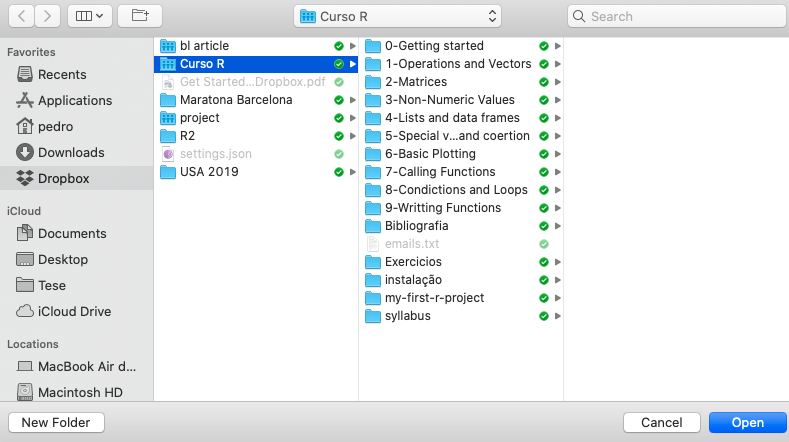
\includegraphics[scale=0.33]{figures/new-project-5.png}
\end{figure}

\end{frame}

\begin{frame}{Your first Rstudio project}
\protect\hypertarget{your-first-rstudio-project-5}{}

\begin{figure}
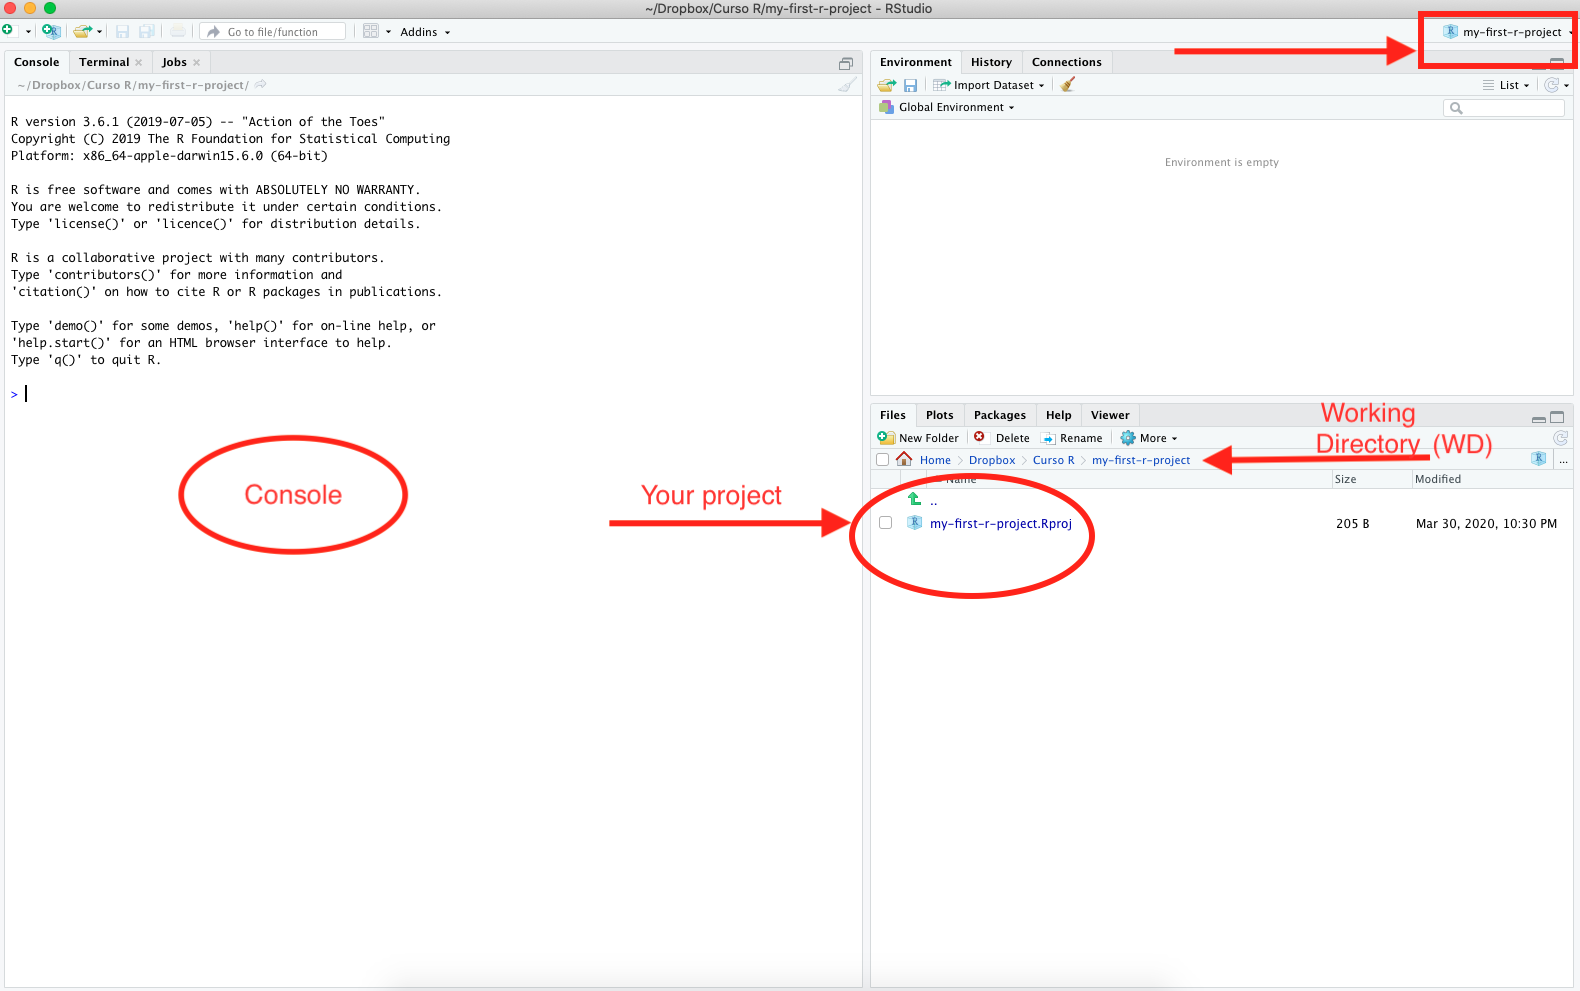
\includegraphics[scale=0.19]{figures/environment.png}
\end{figure}

\end{frame}

\begin{frame}[fragile]{R as a calculator}
\protect\hypertarget{r-as-a-calculator}{}

We can use R's console as a calculator:

\begin{Shaded}
\begin{Highlighting}[]
\DecValTok{2}\OperatorTok{+}\DecValTok{3} 
\end{Highlighting}
\end{Shaded}

\begin{verbatim}
## [1] 5
\end{verbatim}

\begin{Shaded}
\begin{Highlighting}[]
\DecValTok{3}\OperatorTok{*}\DecValTok{5}
\end{Highlighting}
\end{Shaded}

\begin{verbatim}
## [1] 15
\end{verbatim}

\begin{Shaded}
\begin{Highlighting}[]
\FloatTok{14.5}\OperatorTok{/}\DecValTok{6}
\end{Highlighting}
\end{Shaded}

\begin{verbatim}
## [1] 2.416667
\end{verbatim}

\begin{Shaded}
\begin{Highlighting}[]
\DecValTok{3}\OperatorTok{^}\DecValTok{2}
\end{Highlighting}
\end{Shaded}

\begin{verbatim}
## [1] 9
\end{verbatim}

\end{frame}

\begin{frame}[fragile]{R as a calculator}
\protect\hypertarget{r-as-a-calculator-1}{}

\begin{Shaded}
\begin{Highlighting}[]
\NormalTok{(}\DecValTok{3}\OperatorTok{^}\DecValTok{2}\NormalTok{)}\OperatorTok{+}\DecValTok{14}\OperatorTok{/}\NormalTok{(}\DecValTok{6}\OperatorTok{+}\DecValTok{5}\NormalTok{)}
\end{Highlighting}
\end{Shaded}

\begin{verbatim}
## [1] 10.27273
\end{verbatim}

\begin{Shaded}
\begin{Highlighting}[]
\NormalTok{(}\DecValTok{3}\OperatorTok{^}\DecValTok{2}\NormalTok{)}\OperatorTok{+}\DecValTok{14}\OperatorTok{/}\DecValTok{6}\OperatorTok{+}\DecValTok{5}
\end{Highlighting}
\end{Shaded}

\begin{verbatim}
## [1] 16.33333
\end{verbatim}

\end{frame}

\begin{frame}[fragile]{R as a calculator}
\protect\hypertarget{r-as-a-calculator-2}{}

\begin{Shaded}
\begin{Highlighting}[]
\DecValTok{25}\OperatorTok{^}\FloatTok{0.5}
\end{Highlighting}
\end{Shaded}

\begin{verbatim}
## [1] 5
\end{verbatim}

\begin{Shaded}
\begin{Highlighting}[]
\KeywordTok{sqrt}\NormalTok{(}\DecValTok{25}\NormalTok{)}
\end{Highlighting}
\end{Shaded}

\begin{verbatim}
## [1] 5
\end{verbatim}

\end{frame}

\begin{frame}[fragile]{R as a calculator}
\protect\hypertarget{r-as-a-calculator-3}{}

\begin{Shaded}
\begin{Highlighting}[]
\KeywordTok{log}\NormalTok{(}\DecValTok{5}\NormalTok{)}
\end{Highlighting}
\end{Shaded}

\begin{verbatim}
## [1] 1.609438
\end{verbatim}

\begin{Shaded}
\begin{Highlighting}[]
\KeywordTok{log10}\NormalTok{(}\DecValTok{5}\NormalTok{)}
\end{Highlighting}
\end{Shaded}

\begin{verbatim}
## [1] 0.69897
\end{verbatim}

\end{frame}

\begin{frame}[fragile]{R as a calculator}
\protect\hypertarget{r-as-a-calculator-4}{}

\begin{Shaded}
\begin{Highlighting}[]
\NormalTok{pi}
\end{Highlighting}
\end{Shaded}

\begin{verbatim}
## [1] 3.141593
\end{verbatim}

\begin{Shaded}
\begin{Highlighting}[]
\KeywordTok{cos}\NormalTok{(}\DecValTok{2}\OperatorTok{*}\NormalTok{pi)}
\end{Highlighting}
\end{Shaded}

\begin{verbatim}
## [1] 1
\end{verbatim}

\begin{Shaded}
\begin{Highlighting}[]
\KeywordTok{tan}\NormalTok{(}\FloatTok{0.6}\NormalTok{)}
\end{Highlighting}
\end{Shaded}

\begin{verbatim}
## [1] 0.6841368
\end{verbatim}

\begin{Shaded}
\begin{Highlighting}[]
\KeywordTok{sin}\NormalTok{(}\FloatTok{0.6}\NormalTok{)}\OperatorTok{/}\KeywordTok{cos}\NormalTok{(}\FloatTok{0.6}\NormalTok{)}
\end{Highlighting}
\end{Shaded}

\begin{verbatim}
## [1] 0.6841368
\end{verbatim}

\end{frame}

\begin{frame}[fragile]{Functions}
\protect\hypertarget{functions}{}

\begin{itemize}
\item
  R has a large collection of built-in functions.
\item
  We´ve already used \texttt{log}, \texttt{log10}, \texttt{sqrt},
  \texttt{sin}, \texttt{cos} and \texttt{tan}
\end{itemize}

\end{frame}

\begin{frame}[fragile]{Functions}
\protect\hypertarget{functions-1}{}

This is how you call a function:

\begin{Shaded}
\begin{Highlighting}[]
\KeywordTok{function_name}\NormalTok{(}\DataTypeTok{arg1 =}\NormalTok{ val1, }\DataTypeTok{arg2 =}\NormalTok{ val2, ...)}
\end{Highlighting}
\end{Shaded}

\begin{itemize}
\tightlist
\item
  Some arguments are mandatory.
\item
  Some arguments are optional and have default values.
\item
  Argument names are not mandatory.
\item
  If you don't provide the names of the arguments, you must input the
  arguments in the correct order.
\item
  As long as the argument's names are provided, the order is irrelevant.
\item
  Help pages can be useful.
\end{itemize}

\end{frame}

\begin{frame}[fragile]{Getting Help}
\protect\hypertarget{getting-help}{}

\begin{itemize}
\item
  If you don't know what a functions does just put ,``?'', before the
  name of the function and send it to R's console.
\item
  In the help page a function you can find:
\item
  Its arguments and respective admissible values
\item
  The interpretation of its output
\item
  Examples
\item
  Related functions
\end{itemize}

\begin{Shaded}
\begin{Highlighting}[]
\NormalTok{?mean}
\NormalTok{?library}
\NormalTok{?sqrt}
\end{Highlighting}
\end{Shaded}

\end{frame}

\begin{frame}[fragile]{Some examples of functions}
\protect\hypertarget{some-examples-of-functions}{}

The exponential function is given by \texttt{exp()}.

\begin{Shaded}
\begin{Highlighting}[]
\KeywordTok{exp}\NormalTok{(}\DataTypeTok{x=}\DecValTok{3}\NormalTok{)}
\end{Highlighting}
\end{Shaded}

\begin{verbatim}
## [1] 20.08554
\end{verbatim}

\end{frame}

\begin{frame}[fragile]{Some examples of functions}
\protect\hypertarget{some-examples-of-functions-1}{}

Logarithms can be calculated with the \texttt{log} function.

\begin{Shaded}
\begin{Highlighting}[]
\KeywordTok{log}\NormalTok{(}\DataTypeTok{x =} \DecValTok{243}\NormalTok{, }\DataTypeTok{base =} \DecValTok{3}\NormalTok{)}
\end{Highlighting}
\end{Shaded}

\begin{verbatim}
## [1] 5
\end{verbatim}

\begin{Shaded}
\begin{Highlighting}[]
\KeywordTok{log}\NormalTok{(}\DataTypeTok{x =} \DecValTok{243}\NormalTok{)}
\end{Highlighting}
\end{Shaded}

\begin{verbatim}
## [1] 5.493061
\end{verbatim}

The \textit{base} argument is optional. The default value is \(e\).

\end{frame}

\begin{frame}[fragile]{Some examples of functions}
\protect\hypertarget{some-examples-of-functions-2}{}

\begin{Shaded}
\begin{Highlighting}[]
\KeywordTok{log}\NormalTok{(}\DecValTok{243}\NormalTok{, }\KeywordTok{exp}\NormalTok{(}\DecValTok{1}\NormalTok{))}
\end{Highlighting}
\end{Shaded}

\begin{verbatim}
## [1] 5.493061
\end{verbatim}

\begin{Shaded}
\begin{Highlighting}[]
\KeywordTok{log}\NormalTok{(}\KeywordTok{exp}\NormalTok{(}\DecValTok{1}\NormalTok{), }\DecValTok{243}\NormalTok{)}
\end{Highlighting}
\end{Shaded}

\begin{verbatim}
## [1] 0.1820478
\end{verbatim}

\begin{Shaded}
\begin{Highlighting}[]
\KeywordTok{log}\NormalTok{(}\DataTypeTok{base =} \KeywordTok{exp}\NormalTok{(}\DecValTok{1}\NormalTok{), }\DataTypeTok{x =} \DecValTok{243}\NormalTok{)}
\end{Highlighting}
\end{Shaded}

\begin{verbatim}
## [1] 5.493061
\end{verbatim}

Tip: try

\begin{Shaded}
\begin{Highlighting}[]
\NormalTok{?log}
\end{Highlighting}
\end{Shaded}

\end{frame}

\begin{frame}[fragile]{Some examples of functions}
\protect\hypertarget{some-examples-of-functions-3}{}

\begin{Shaded}
\begin{Highlighting}[]
\KeywordTok{log}\NormalTok{(}\DataTypeTok{x =} \DecValTok{243}\NormalTok{, }\DataTypeTok{base =} \KeywordTok{exp}\NormalTok{(}\DecValTok{1}\NormalTok{))}
\end{Highlighting}
\end{Shaded}

\begin{verbatim}
## [1] 5.493061
\end{verbatim}

\begin{Shaded}
\begin{Highlighting}[]
\KeywordTok{log10}\NormalTok{(}\DecValTok{5}\NormalTok{)}
\end{Highlighting}
\end{Shaded}

\begin{verbatim}
## [1] 0.69897
\end{verbatim}

\begin{Shaded}
\begin{Highlighting}[]
\DecValTok{2}\OperatorTok{^}\KeywordTok{log2}\NormalTok{(}\DecValTok{6}\NormalTok{)}
\end{Highlighting}
\end{Shaded}

\begin{verbatim}
## [1] 6
\end{verbatim}

\begin{Shaded}
\begin{Highlighting}[]
\DecValTok{10}\OperatorTok{^}\KeywordTok{log10}\NormalTok{(}\DecValTok{5}\NormalTok{)}\OperatorTok{+}\DecValTok{1}
\end{Highlighting}
\end{Shaded}

\begin{verbatim}
## [1] 6
\end{verbatim}

\end{frame}

\begin{frame}{R scripts}
\protect\hypertarget{r-scripts}{}

\begin{itemize}
\item
  We´ve been using R's console
\item
  Code sent directly to the console is executed but you won't be able to
  modify it or reuse it later
\item
  Writting our code in scripts is a better option
\item
  A script is just a text file we can use to write code
\end{itemize}

\end{frame}

\begin{frame}{Your first R script}
\protect\hypertarget{your-first-r-script}{}

\begin{figure}
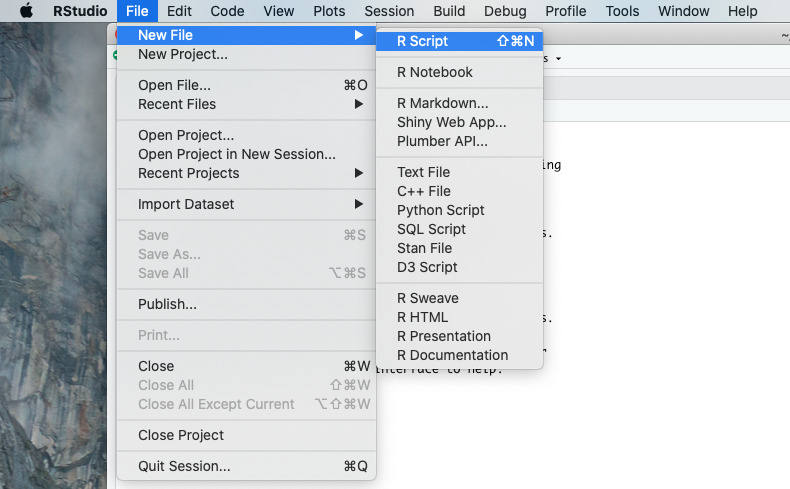
\includegraphics[scale=0.35]{figures/new-script.png}
\end{figure}

\end{frame}

\begin{frame}{Rstudio Panes}
\protect\hypertarget{rstudio-panes}{}

\begin{figure}
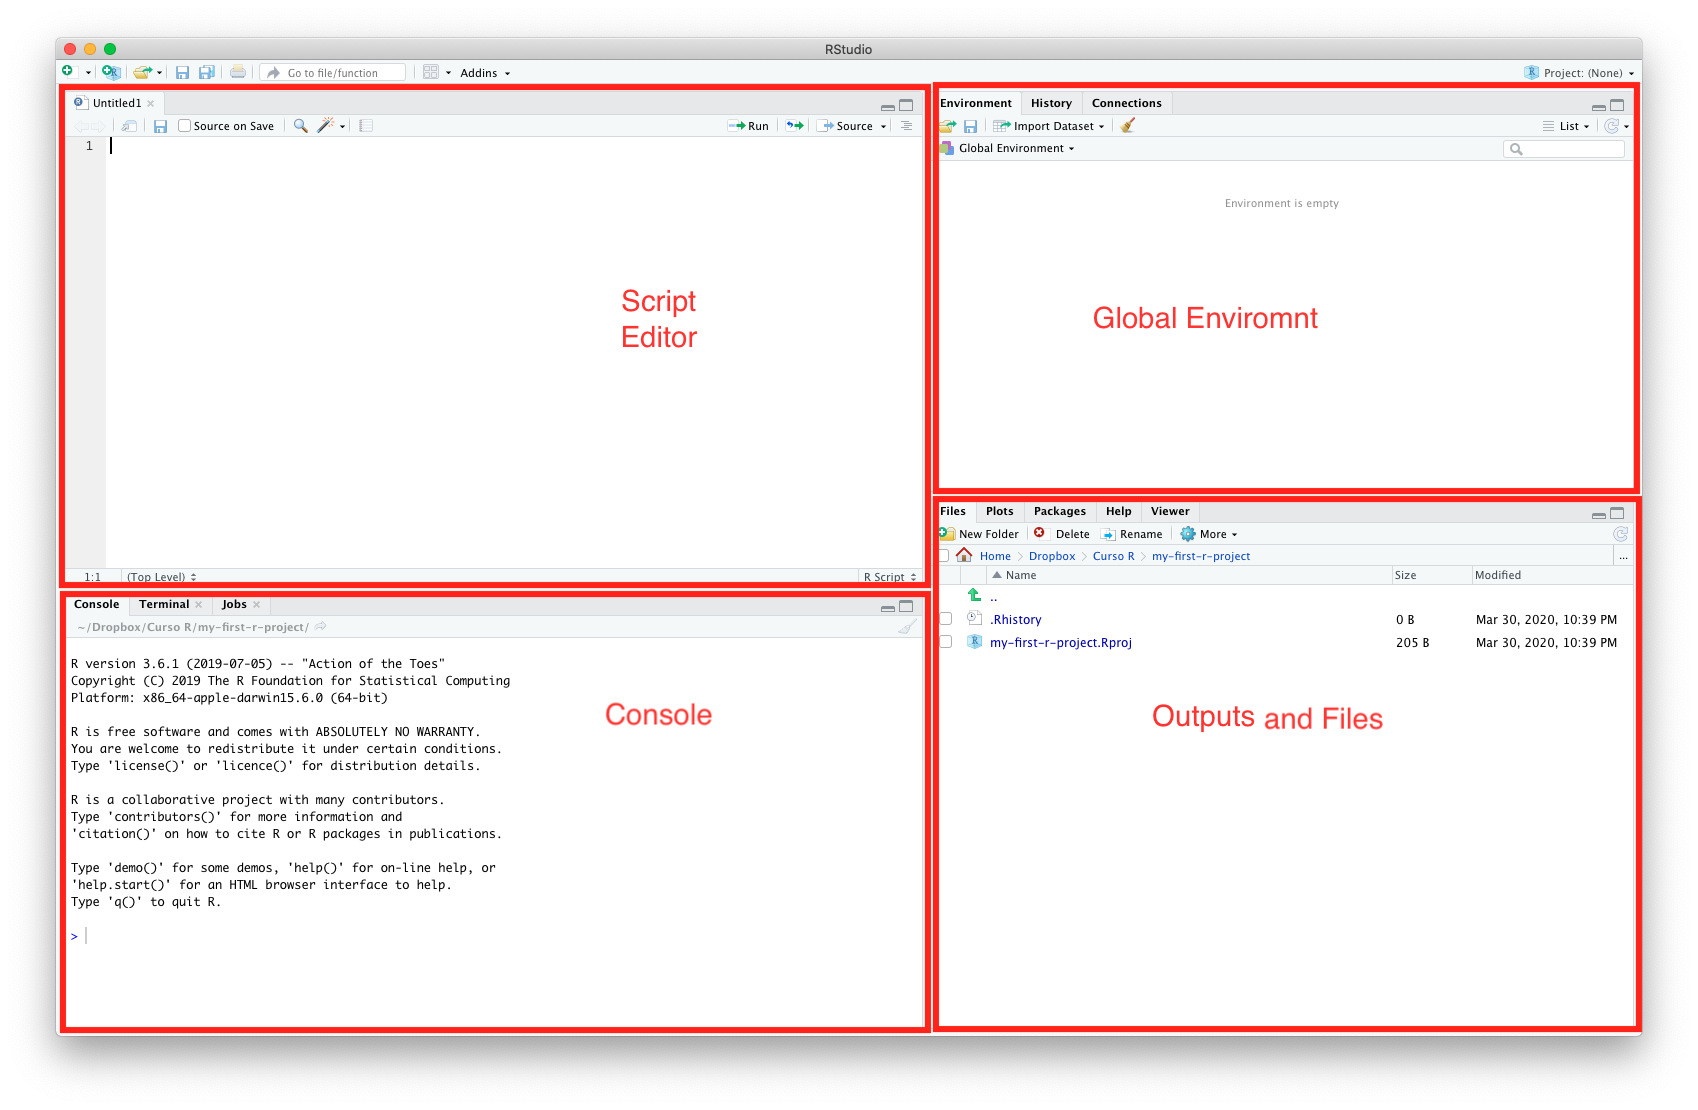
\includegraphics[scale=0.18]{figures/panes.png}
\end{figure}

\end{frame}

\begin{frame}{Editor}
\protect\hypertarget{editor}{}

\begin{itemize}
\tightlist
\item
  R opens scripts in the editor pane
\item
  This is where you should write your code
\item
  In the editor you can modify, rerun and save your code at any time
\end{itemize}

\end{frame}

\begin{frame}{Some Useful Shortcuts}
\protect\hypertarget{some-useful-shortcuts}{}

\begin{itemize}
\item
  New script: Cmd/Ctrl + Shift + N
\item
  Save the script: Cmd/Ctrl + S
\item
  Send code from the editor to the console:

  \begin{itemize}
  \tightlist
  \item
    Cmd/Ctrl + Enter (current line or current selection)
  \item
    Cmd/Ctrl + Shift + S (entire script)
  \end{itemize}
\end{itemize}

\end{frame}

\begin{frame}{More Shortcuts}
\protect\hypertarget{more-shortcuts}{}

\begin{itemize}
\item
  To see a list of Rstudio shortcuts try: Alt/Option + Shift + k
\item
  Alternative: click
  \href{https://support.rstudio.com/hc/en-us/articles/200711853-Keyboard-Shortcuts}{here}
\end{itemize}

\end{frame}

\begin{frame}[fragile]{Assigning values to objects}
\protect\hypertarget{assigning-values-to-objects}{}

To store values in R's memory you need to assign them to objects. You
can use the equal sign, the assign function, or the assign operator:

\begin{itemize}
\tightlist
\item
  The assignment operator is typically recommended.
\item
  The equal sign should be reserved to provide arguments to functions.
\end{itemize}

\begin{Shaded}
\begin{Highlighting}[]
\NormalTok{object_name_}\DecValTok{1}\NormalTok{ <-}\StringTok{ }\DecValTok{5}
\NormalTok{object_name_}\DecValTok{1}
\end{Highlighting}
\end{Shaded}

\begin{verbatim}
## [1] 5
\end{verbatim}

\begin{Shaded}
\begin{Highlighting}[]
\NormalTok{object_name_}\DecValTok{2}\NormalTok{ <-}\StringTok{ }\KeywordTok{log}\NormalTok{(object_name_}\DecValTok{1}\NormalTok{) }\OperatorTok{+}\StringTok{ }\KeywordTok{exp}\NormalTok{(}\DecValTok{5}\NormalTok{)}
\NormalTok{object_name_}\DecValTok{2}
\end{Highlighting}
\end{Shaded}

\begin{verbatim}
## [1] 150.0226
\end{verbatim}

Rstudio's keyboard shortcut for the assign operator: ``Alt/Option'' +
``\(-\)''

\end{frame}

\begin{frame}{The assignment operator}
\protect\hypertarget{the-assignment-operator}{}


\includegraphics[scale=.22]{figures/meme.jpg}

\end{frame}

\begin{frame}{The assignment operator}
\protect\hypertarget{the-assignment-operator-1}{}

\begin{figure}
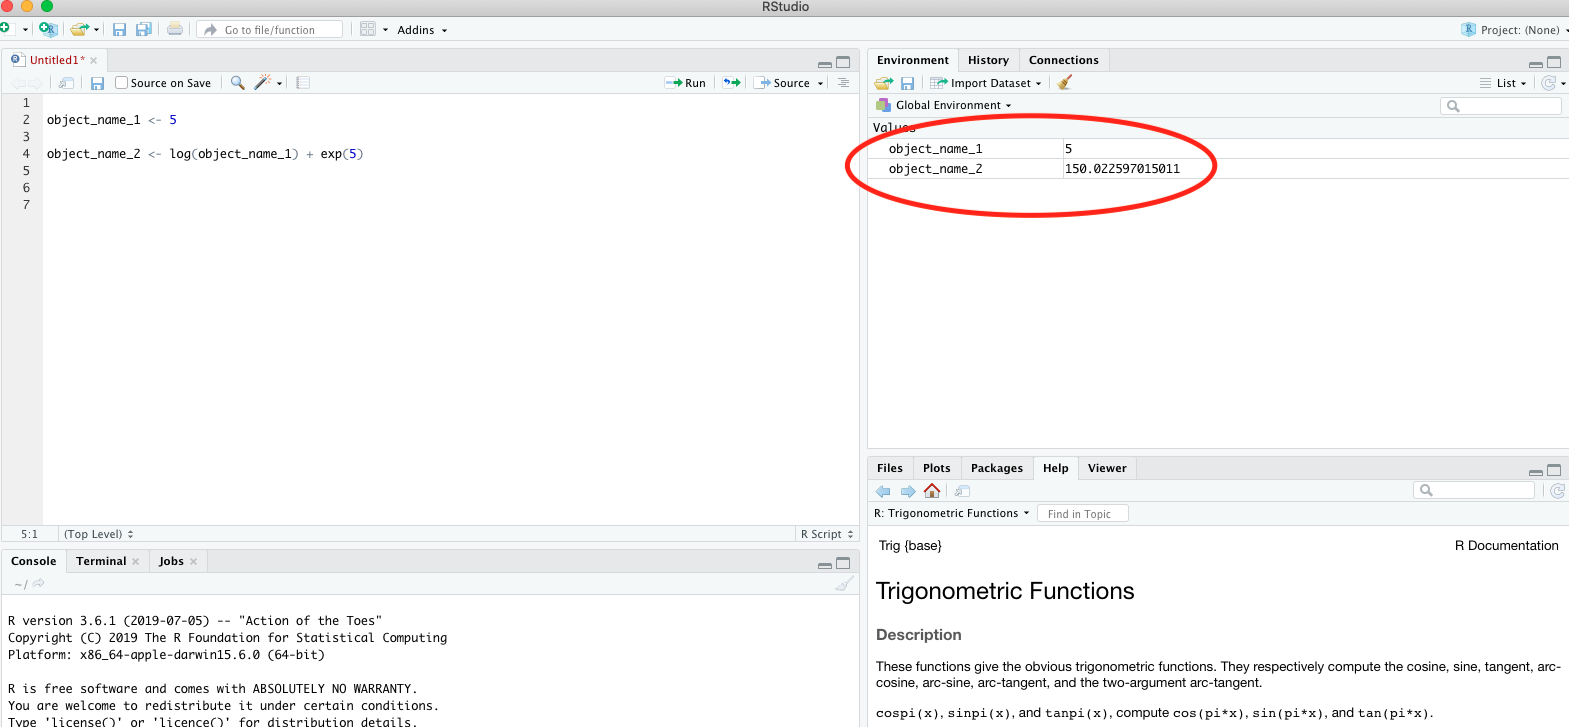
\includegraphics[scale=.19]{figures/objects.png}
\caption{Stored objects are visible in the upper-right pane, under the "Environment" tab}
\end{figure}

\end{frame}

\begin{frame}{Example}
\protect\hypertarget{example}{}

\begin{figure}
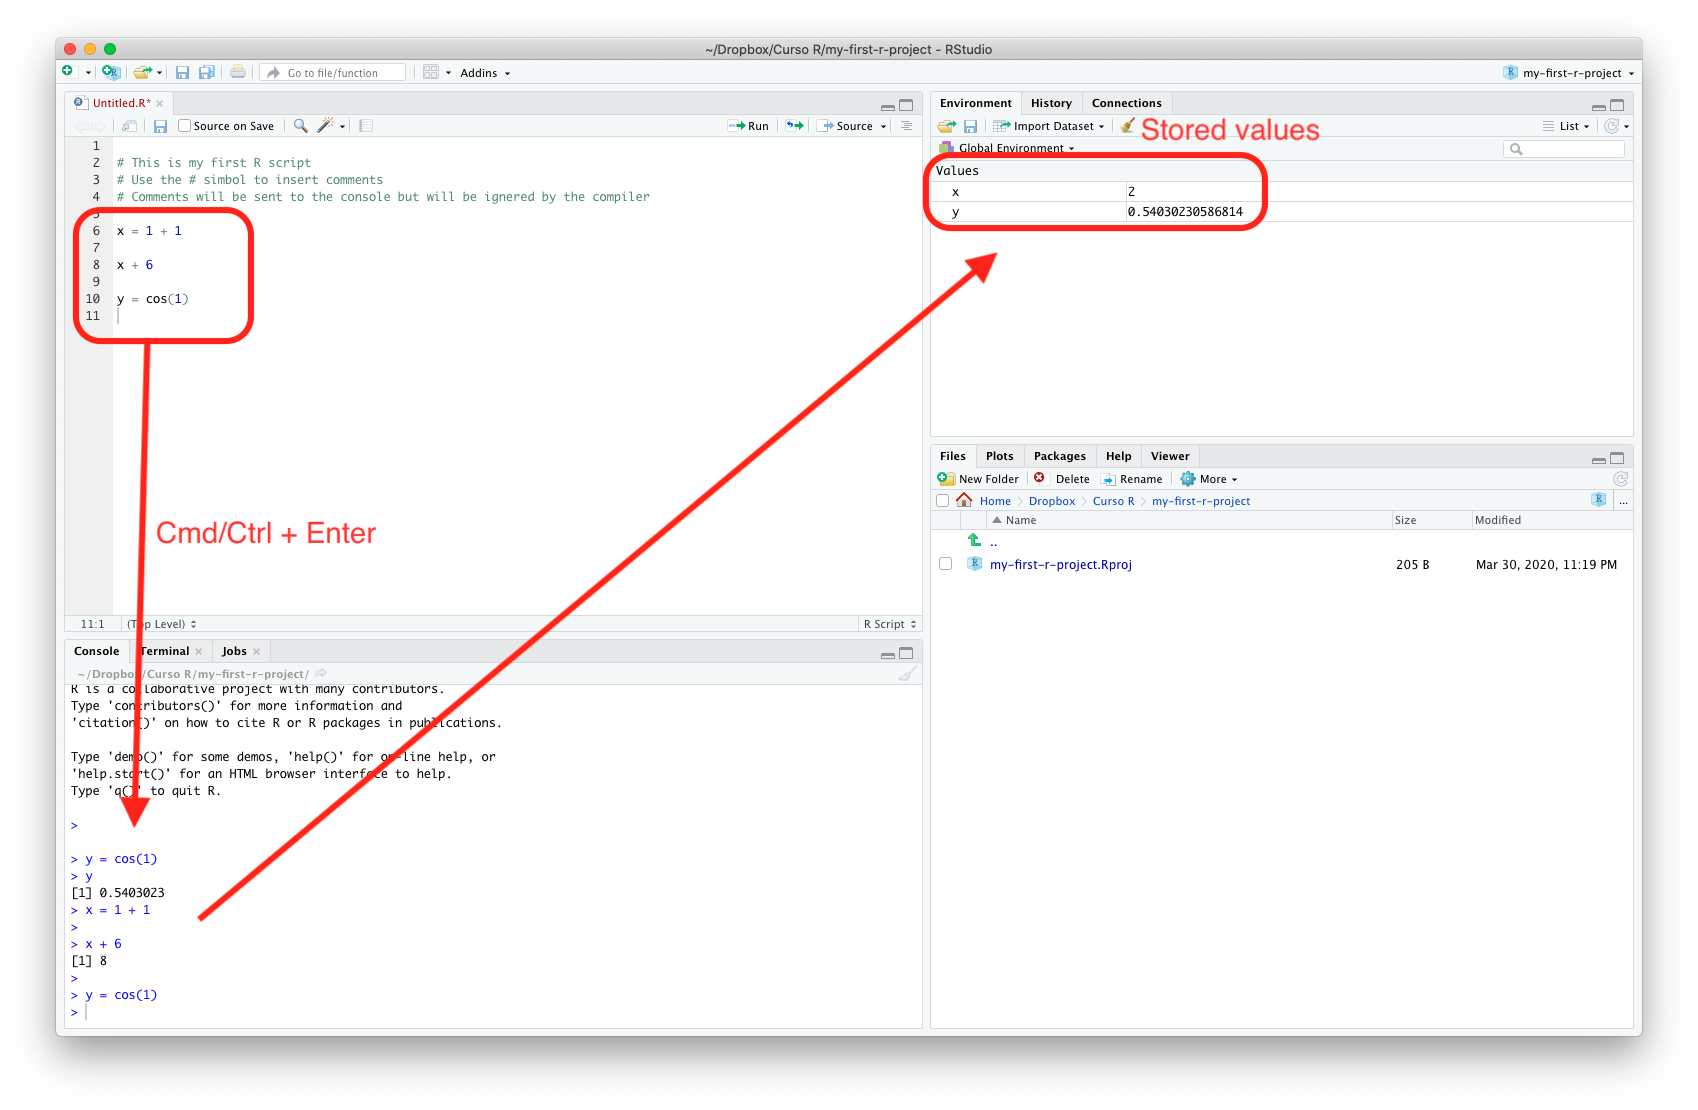
\includegraphics[scale=0.17]{figures/edit-script.png}
\end{figure}

\end{frame}

\begin{frame}{Example (cont.)}
\protect\hypertarget{example-cont.}{}

\begin{figure}
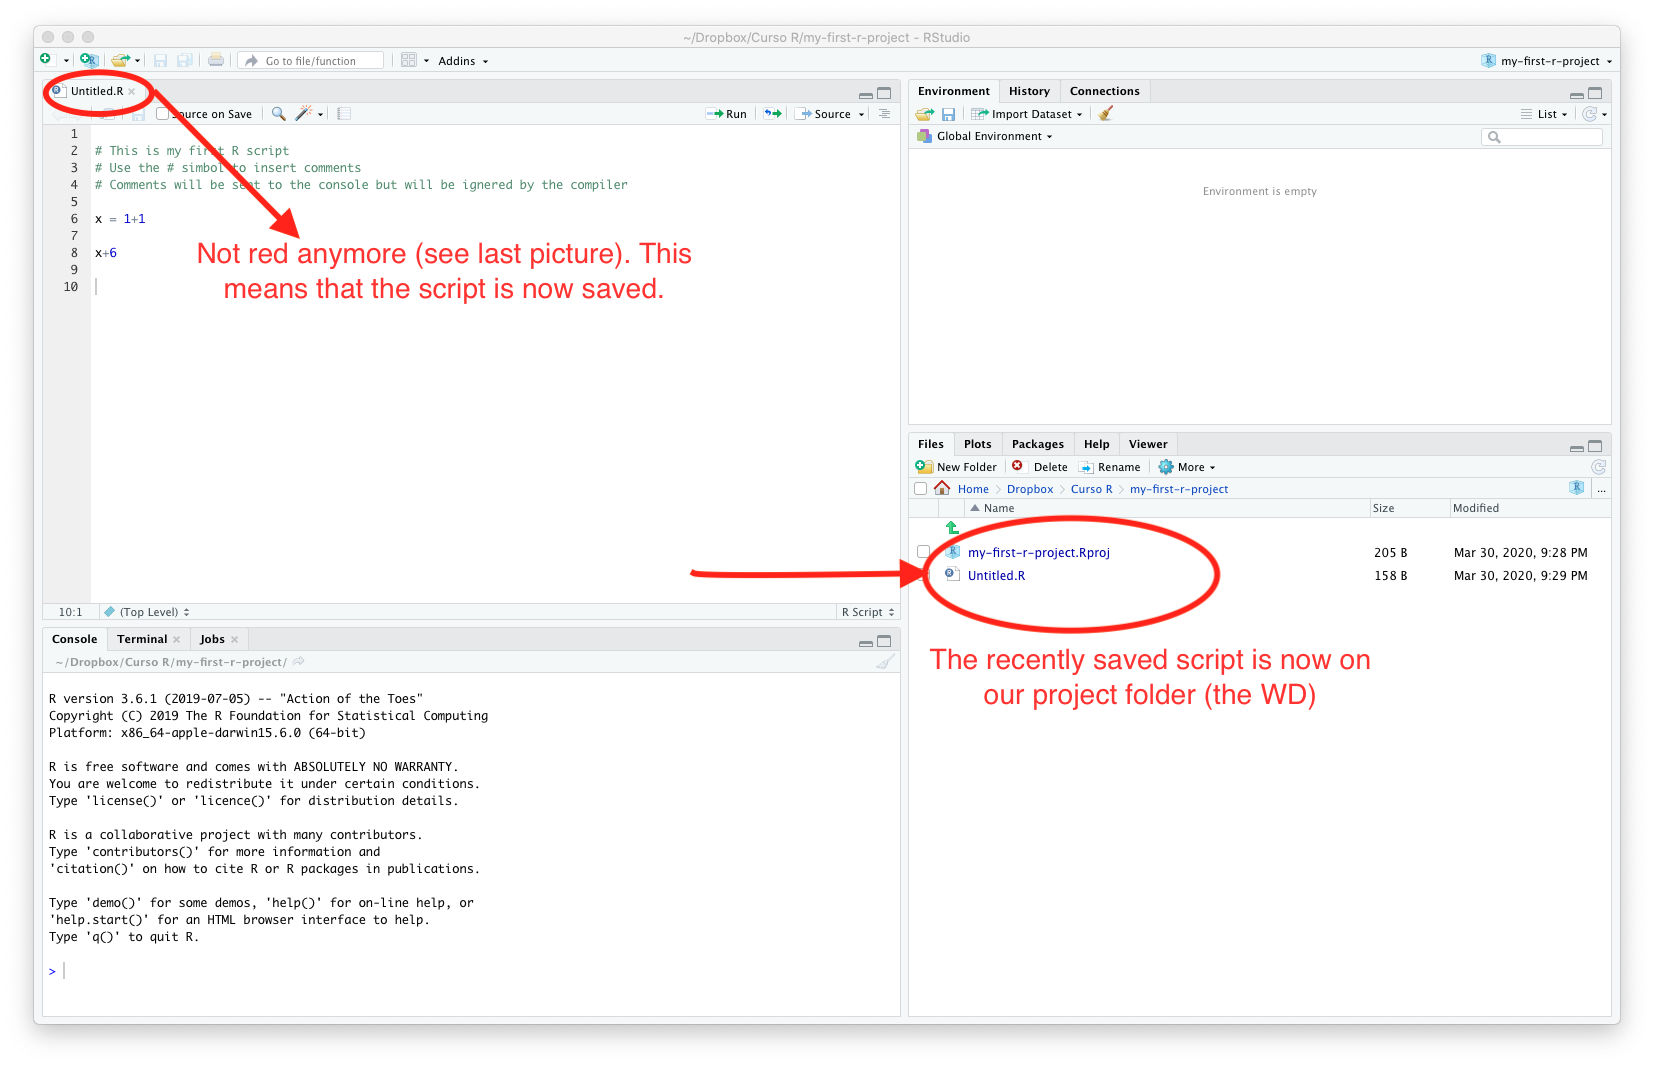
\includegraphics[scale=0.17]{figures/saved-script.png}
\end{figure}

\end{frame}

\begin{frame}{Naming Objects}
\protect\hypertarget{naming-objects}{}

Object names must start with a letter and can only contain letters,
numbers, underscores and dots. You want your object names to be short,
descriptive and consistent. Ideally, one should follow a convention:

\begin{itemize}
\tightlist
\item
  i\_use\_snake\_case
\item
  otherPeopleUseCamelCase
\item
  some.people.use.periods
\item
  And\_aFew.People\_RENOUNCEconvention
\end{itemize}

\end{frame}

\begin{frame}[fragile]{Case Matters}
\protect\hypertarget{case-matters}{}

\begin{Shaded}
\begin{Highlighting}[]
\NormalTok{pi}
\end{Highlighting}
\end{Shaded}

\begin{verbatim}
## [1] 3.141593
\end{verbatim}

\begin{Shaded}
\begin{Highlighting}[]
\NormalTok{r_rocks <-}\StringTok{ }\DecValTok{2} \OperatorTok{*}\StringTok{ }\NormalTok{pi}\OperatorTok{^}\DecValTok{2}
\NormalTok{r_rocks}
\end{Highlighting}
\end{Shaded}

\begin{verbatim}
## [1] 19.73921
\end{verbatim}

\begin{Shaded}
\begin{Highlighting}[]
\NormalTok{r_Rocks}
\end{Highlighting}
\end{Shaded}

\begin{verbatim}
## Error in eval(expr, envir, enclos): object 'r_Rocks' not found
\end{verbatim}

\end{frame}

\begin{frame}[fragile]{How to delete objects}
\protect\hypertarget{how-to-delete-objects}{}

To delete stored objects use the \texttt{rm} function:

\begin{Shaded}
\begin{Highlighting}[]
\KeywordTok{rm}\NormalTok{(object_name_}\DecValTok{1}\NormalTok{)}
\NormalTok{object_name_}\DecValTok{1}
\end{Highlighting}
\end{Shaded}

\begin{verbatim}
## Error in eval(expr, envir, enclos): object 'object_name_1' not found
\end{verbatim}

\end{frame}

\begin{frame}[fragile]{How to delete objects}
\protect\hypertarget{how-to-delete-objects-1}{}

\begin{itemize}
\item
  You can input as many objects as you want to \texttt{rm()}
\item
  To remove all stored objects all once, use the following command:
\end{itemize}

\begin{Shaded}
\begin{Highlighting}[]
\KeywordTok{rm}\NormalTok{(}\DataTypeTok{list =} \KeywordTok{ls}\NormalTok{())}
\end{Highlighting}
\end{Shaded}

\end{frame}

\begin{frame}[fragile]{How to print the assigned value}
\protect\hypertarget{how-to-print-the-assigned-value}{}

If you make an assignment, you don't get to see the assigned value.
You're then tempted to double-check the result:

\begin{Shaded}
\begin{Highlighting}[]
\NormalTok{y <-}\StringTok{ }\KeywordTok{log}\NormalTok{(}\DecValTok{2}\NormalTok{)}\OperatorTok{+}\DecValTok{1}
\NormalTok{y}
\end{Highlighting}
\end{Shaded}

\begin{verbatim}
## [1] 1.693147
\end{verbatim}

This common action can be shortened by surrounding the assignment with
parentheses, which causes assignments to print:

\begin{Shaded}
\begin{Highlighting}[]
\NormalTok{(y <-}\StringTok{ }\KeywordTok{log}\NormalTok{(}\DecValTok{2}\NormalTok{)}\OperatorTok{+}\DecValTok{1}\NormalTok{)}
\end{Highlighting}
\end{Shaded}

\begin{verbatim}
## [1] 1.693147
\end{verbatim}

\end{frame}

\begin{frame}[fragile]{Overwritting stored values}
\protect\hypertarget{overwritting-stored-values}{}

\begin{Shaded}
\begin{Highlighting}[]
\NormalTok{x <-}\StringTok{ }\DecValTok{-5}
\NormalTok{x}
\end{Highlighting}
\end{Shaded}

\begin{verbatim}
## [1] -5
\end{verbatim}

\begin{Shaded}
\begin{Highlighting}[]
\NormalTok{x <-}\StringTok{ }\NormalTok{x }\OperatorTok{+}\StringTok{ }\DecValTok{1} 
\NormalTok{x}
\end{Highlighting}
\end{Shaded}

\begin{verbatim}
## [1] -4
\end{verbatim}

\end{frame}

\begin{frame}{Working directory}
\protect\hypertarget{working-directory}{}

An active R session always has an associated working directory. R will
use the working directory by default to:

\begin{itemize}
\tightlist
\item
  Search for files
\item
  Save outputs (tables, plots, etc)
\end{itemize}

\end{frame}

\begin{frame}{Setting the working directory}
\protect\hypertarget{setting-the-working-directory}{}

\begin{figure}
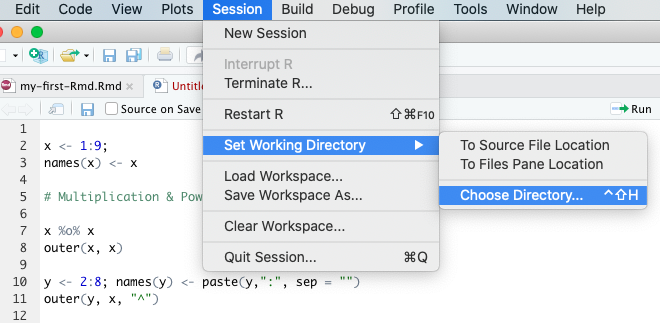
\includegraphics[scale = .38]{figures/wd}
\caption{Setting the working directory}
\end{figure}

\end{frame}

\begin{frame}[fragile]{Setting and setting the working directory}
\protect\hypertarget{setting-and-setting-the-working-directory}{}

You can also get or set the working directory in R's console:

\begin{Shaded}
\begin{Highlighting}[]
\KeywordTok{getwd}\NormalTok{()}
\end{Highlighting}
\end{Shaded}

\begin{Shaded}
\begin{Highlighting}[]
\KeywordTok{setwd}\NormalTok{(}\StringTok{"/folder1/folder2/folder3/"}\NormalTok{)}
\end{Highlighting}
\end{Shaded}

\begin{itemize}
\tightlist
\item
  The problem with commands like this is that such paths will only exist
  on your computer
\item
  Solution: Rstudio projects
\end{itemize}

\end{frame}

\begin{frame}[fragile]{Advantages of Rstudio projects}
\protect\hypertarget{advantages-of-rstudio-projects}{}

\begin{itemize}
\tightlist
\item
  Rstudio projects are self-contained.
\item
  They put together all the files that are relevant for a particular
  project (article, book, research project) in the same folder.
\item
  The project's working directory always points to that folder by
  default
\item
  Rstudio projects can be moved around on your computer or onto other
  computers and will still ``just work''. No directory changes are
  needed.
\item
  If you need to create additional folders or start moving around parts
  of you project around dont use the \texttt{setwd} function. It is
  safer to reference the full path.
\end{itemize}

\end{frame}

\begin{frame}[fragile]{Packages}
\protect\hypertarget{packages}{}

\begin{itemize}
\item
  The more specialized functions and data sets are available on packages
  (also referred to as libraries).
\item
  Installing R Packages:
\end{itemize}

\begin{Shaded}
\begin{Highlighting}[]
\KeywordTok{install.packages}\NormalTok{(}\StringTok{"ggplot2"}\NormalTok{, }\DataTypeTok{dependencies =} \OtherTok{TRUE}\NormalTok{)}
\end{Highlighting}
\end{Shaded}

Loading R Packages:

\begin{Shaded}
\begin{Highlighting}[]
\KeywordTok{library}\NormalTok{(}\StringTok{"ggplot2"}\NormalTok{)}
\end{Highlighting}
\end{Shaded}

Updating R Packages:

\begin{Shaded}
\begin{Highlighting}[]
\KeywordTok{update.packages}\NormalTok{()  }\CommentTok{# This is rarely necessary }
\end{Highlighting}
\end{Shaded}

\begin{itemize}
\tightlist
\item
  Packages are developed by the R core team and also by the community of
  R users.
\item
  You can develop your own packages and make them available to the
  community on \href{https://cran.r-project.org}{CRAN}(The Comprehensive
  R Archive Network)
\end{itemize}

\end{frame}

\begin{frame}[fragile]{Packages}
\protect\hypertarget{packages-1}{}

\begin{itemize}
\tightlist
\item
  It is typically recommend to start your scripts with the packages that
  you need.
\item
  That way, if you share your code with others, they can easily see what
  packages they need to install.
\item
  Note, however, that you should never include \texttt{install.packages}
  or \texttt{setwd} in a script that you share.
\item
  It is very antisocial to change settings on someone else's computer!
\end{itemize}

\end{frame}

\begin{frame}{Settings}
\protect\hypertarget{settings}{}

You can change Rstudio's default settings and appearence:

\begin{itemize}
\tightlist
\item
  Mac: Tools \(->\) Global Option
\item
  Windows and Linux: Rstudio \(->\) preferences
\end{itemize}

Shortcut:

\begin{itemize}
\tightlist
\item
  Mac: ``Cmd'' + ``,''
\item
  Windows and Linux: ``Ctrl'' + ``,''
\end{itemize}

\end{frame}

\begin{frame}{Settings}
\protect\hypertarget{settings-1}{}

\begin{figure}
   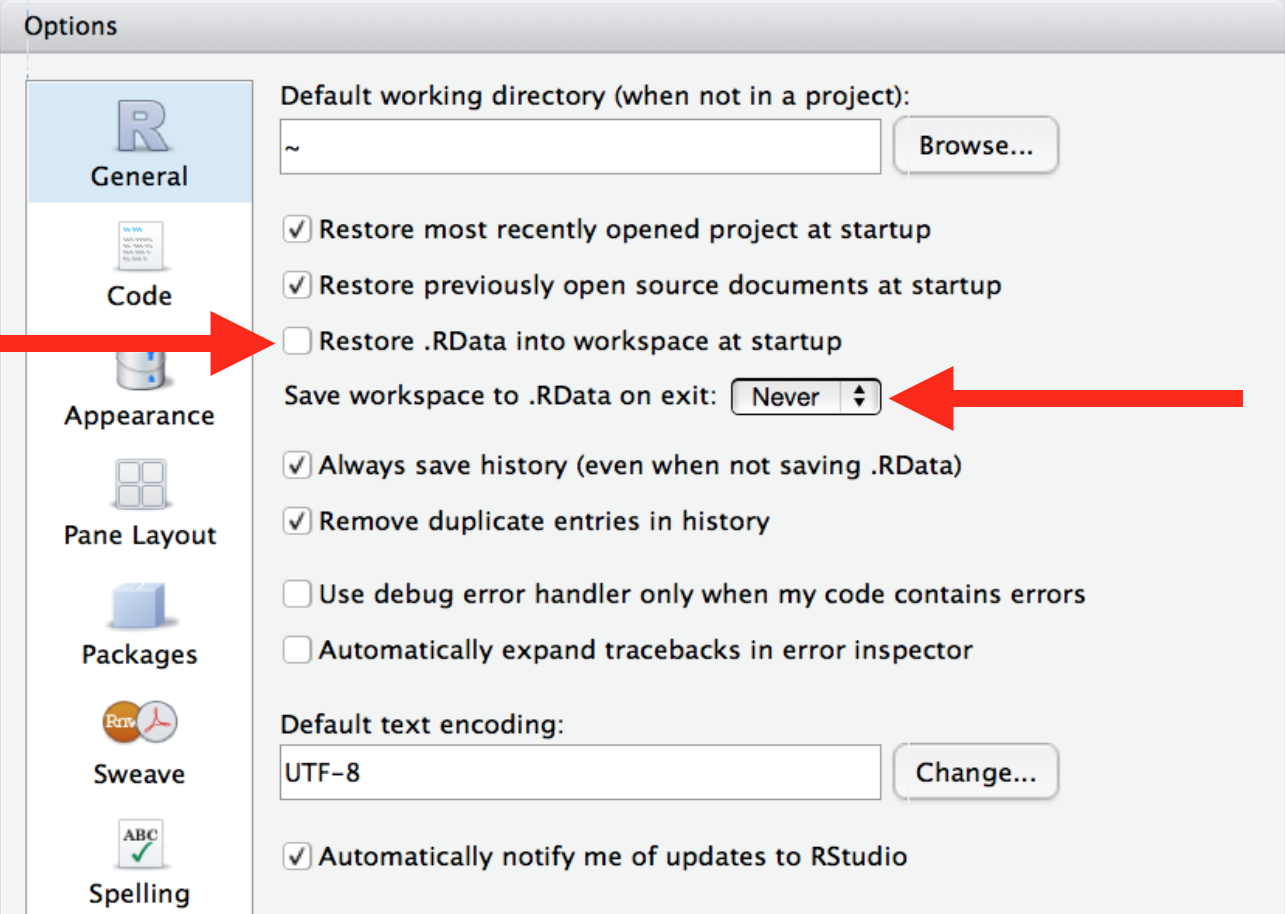
\includegraphics[scale = .3]{figures/settings.png}
   \caption{These are the general settings that we recommend}
\end{figure}

\end{frame}

\begin{frame}{Settings}
\protect\hypertarget{settings-2}{}

\begin{figure}
   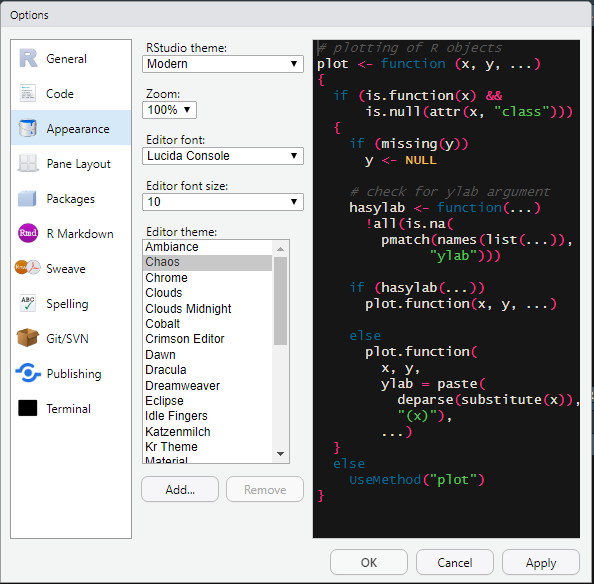
\includegraphics[scale = .35]{figures/Screenshot_4}
   \caption{Changing Rstudio's appearence}
\end{figure}

\end{frame}

\end{document}
